%%%%%%%%%%%%%%%%%%%%%%%%%%%%%%%%%%%%%%%%%%%%%%%%%%%%%%%%%%%%
% 2.2 ANALYTIC NUMBER THEORY
% The Composition of Advanced Mathematics
%%%%%%%%%%%%%%%%%%%%%%%%%%%%%%%%%%%%%%%%%%%%%%%%%%%%%%%%%%%%

\section{Analytic Number Theory}
\label{sec:analytic-number-theory}

\prerequisite{
Elementary Number Theory from \cref{sec:elementary-number-theory}, together
with familiarity with functions, limits, logarithms, infinite series, and
basic calculus. More advanced parts of this section use ideas developed
systematically in Chapter 5 on Analysis.
}

\learningobjectives{
By the end of this section, the reader should be able to:
\begin{itemize}
    \item explain the central goals of analytic number theory;
    \item describe the distribution of prime numbers using counting functions;
    \item work with the prime-counting function \(\pi(x)\);
    \item interpret the Prime Number Theorem;
    \item compare \(\pi(x)\) with elementary approximations such as \(x/\log x\);
    \item work with arithmetic functions such as \(\mu(n)\), \(\Lambda(n)\), and \(d(n)\);
    \item understand multiplicative arithmetic functions;
    \item use Dirichlet convolution;
    \item apply the Möbius inversion formula;
    \item understand Dirichlet series as generating objects for arithmetic functions;
    \item explain the Euler product for the Riemann zeta function;
    \item identify the relationship between the zeta function and prime numbers;
    \item understand the basic role of analytic continuation and zeros of \(\zeta(s)\);
    \item state the Riemann Hypothesis and explain its significance without assuming it is true;
    \item understand the basic idea of primes in arithmetic progressions;
    \item work with Dirichlet characters at an introductory level;
    \item understand the purpose of Dirichlet \(L\)-functions;
    \item recognize common summation and asymptotic notation;
    \item apply elementary analytic estimates to arithmetic sums;
    \item understand how analytic methods reveal large-scale patterns in the integers.
\end{itemize}
}

%%%%%%%%%%%%%%%%%%%%%%%%%%%%%%%%%%%%%%%%%%%%%%%%%%%%%%%%%%%%
\subsection{What Is Analytic Number Theory?}
\label{subsec:what-is-analytic-number-theory}
%%%%%%%%%%%%%%%%%%%%%%%%%%%%%%%%%%%%%%%%%%%%%%%%%%%%%%%%%%%%

Elementary number theory studies discrete arithmetic objects such as primes,
divisors, congruences, and Diophantine equations. Analytic number theory
studies many of the same objects using methods from analysis.

\begin{definitionbox}{Analytic Number Theory}
\emph{Analytic number theory} is the branch of number theory that applies
methods from real analysis, complex analysis, infinite series, asymptotic
analysis, and related areas to study integers and arithmetic functions.
\end{definitionbox}

One of its central questions is deceptively simple:

\begin{center}
\emph{How are the prime numbers distributed among the positive integers?}
\end{center}

The primes

\[ 2,3,5,7,11,13,17,19,23,29,\ldots \]

do not occur at regular intervals. Nevertheless, their large-scale
distribution follows remarkably precise analytic laws.

\begin{conceptbox}
Analytic number theory replaces the question

\[
\text{``Where is the next prime?''}
\]

with broader questions such as

\[
\text{``Approximately how many primes occur below }x\text{?''}
\]

and

\[
\text{``How large is the error in that approximation?''}
\]

The shift from exact individual values to global behavior is one of the
central ideas of the subject.
\end{conceptbox}

%%%%%%%%%%%%%%%%%%%%%%%%%%%%%%%%%%%%%%%%%%%%%%%%%%%%%%%%%%%%
\subsection{Arithmetic Functions}
\label{subsec:analytic-arithmetic-functions}
%%%%%%%%%%%%%%%%%%%%%%%%%%%%%%%%%%%%%%%%%%%%%%%%%%%%%%%%%%%%

An important tool in number theory is a function whose inputs are positive
integers.

\begin{definitionbox}{Arithmetic Function}
An \emph{arithmetic function}, also called a \emph{number-theoretic
function}, is a function

\[ f:\N\to\C. \]
\end{definitionbox}

The codomain may be restricted to \(\R\), \(\Z\), or another set when
appropriate.

Examples already encountered include Euler's phi function

\[ \varphi(n), \]

the divisor-counting function

\[ \tau(n), \]

and the divisor-sum function

\[ \sigma(n). \]

Analytic number theory studies both the exact values and the average behavior
of such functions.

%%%%%%%%%%%%%%%%%%%%%%%%%%%%%%%%%%%%%%%%%%%%%%%%%%%%%%%%%%%%
\subsection{The Prime-Counting Function}
\label{subsec:prime-counting-function}
%%%%%%%%%%%%%%%%%%%%%%%%%%%%%%%%%%%%%%%%%%%%%%%%%%%%%%%%%%%%

The most basic analytic description of the primes is obtained by counting
them.

\begin{definitionbox}{Prime-Counting Function}
For \(x\geq0\), the \emph{prime-counting function} is

\[ \pi(x)=\#\{p\leq x:p\text{ is prime}\}. \]
\end{definitionbox}

The Greek letter

\[ \pi \]

is called \emph{pi}, pronounced ``pie.''

In this context, \(\pi(x)\) does not represent the geometric constant
\(3.14159\ldots\). Instead, it counts primes.

The symbol

\[ \#S \]

means the \emph{cardinality} or number of elements of the set \(S\).

Thus

\[ \pi(10)=4 \]

because the primes not exceeding \(10\) are

\[ 2,3,5,7. \]

Similarly,

\[ \pi(100)=25. \]

%%%%%%%%%%%%%%%%%%%%%%%%%%%%%%%%%%%%%%%%%%%%%%%%%%%%%%%%%%%%
\subsection{Visualizing the Prime-Counting Function}
\label{subsec:visualizing-prime-counting}
%%%%%%%%%%%%%%%%%%%%%%%%%%%%%%%%%%%%%%%%%%%%%%%%%%%%%%%%%%%%

The function \(\pi(x)\) is a step function. It increases by one whenever
\(x\) passes a prime number.

\begin{centereddiagram}
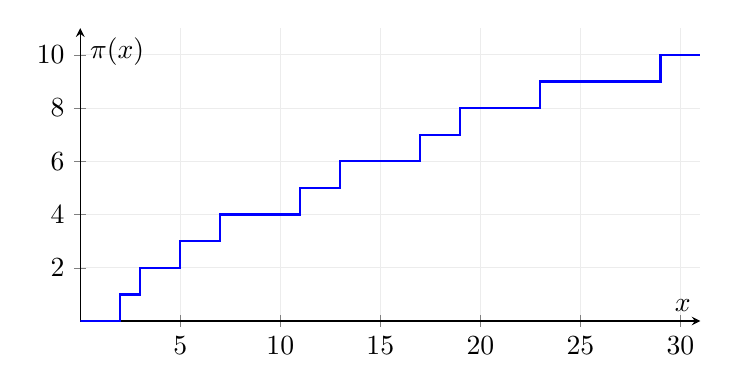
\begin{tikzpicture}
\begin{axis}[
    width=0.78\textwidth,
    height=5.3cm,
    axis lines=middle,
    xmin=0,
    xmax=31,
    ymin=0,
    ymax=11,
    xlabel={$x$},
    ylabel={$\pi(x)$},
    xtick={0,5,10,15,20,25,30},
    ytick={0,2,4,6,8,10},
    grid=both,
    grid style={gray!15}
]
\addplot+[const plot,no marks,thick] coordinates {
    (0,0)
    (2,1)
    (3,2)
    (5,3)
    (7,4)
    (11,5)
    (13,6)
    (17,7)
    (19,8)
    (23,9)
    (29,10)
    (31,10)
};
\end{axis}
\end{tikzpicture}
\end{centereddiagram}

The irregular spacing of the jumps reflects the irregular spacing of the
prime numbers.

%%%%%%%%%%%%%%%%%%%%%%%%%%%%%%%%%%%%%%%%%%%%%%%%%%%%%%%%%%%%
\subsection{Prime Density}
\label{subsec:prime-density}
%%%%%%%%%%%%%%%%%%%%%%%%%%%%%%%%%%%%%%%%%%%%%%%%%%%%%%%%%%%%

As integers become larger, primes become less frequent.

A useful informal measure of prime density near \(x\) is

\[ \frac{1}{\log x}. \]

Here \(\log x\) denotes the natural logarithm.

This suggests that the number of primes up to \(x\) should be approximately

\[ \frac{x}{\log x}. \]

This approximation is the starting point for one of the most important
theorems in mathematics.

%%%%%%%%%%%%%%%%%%%%%%%%%%%%%%%%%%%%%%%%%%%%%%%%%%%%%%%%%%%%
\subsection{Asymptotic Equivalence}
\label{subsec:asymptotic-equivalence-number-theory}
%%%%%%%%%%%%%%%%%%%%%%%%%%%%%%%%%%%%%%%%%%%%%%%%%%%%%%%%%%%%

Analytic number theory frequently compares functions as their arguments
become large.

\begin{definitionbox}{Asymptotic Equivalence}
Let \(f(x)\) and \(g(x)\) be positive functions for sufficiently large \(x\).
We write

\[ f(x)\sim g(x)\qquad(x\to\infty) \]

if

\[ \lim_{x\to\infty}\frac{f(x)}{g(x)}=1. \]
\end{definitionbox}

The symbol

\[ \sim \]

is called the \emph{asymptotic equivalence symbol} in this context.

The statement

\[ f(x)\sim g(x) \]

is read

\begin{center}
``\(f(x)\) is asymptotic to \(g(x)\).''
\end{center}

It means that the relative error between the two quantities approaches zero.

\begin{warningbox}
Asymptotic equivalence does not mean that two functions become equal.

The statement

\[ f(x)\sim g(x) \]

describes their relative growth as \(x\to\infty\).
\end{warningbox}

%%%%%%%%%%%%%%%%%%%%%%%%%%%%%%%%%%%%%%%%%%%%%%%%%%%%%%%%%%%%
\subsection{The Prime Number Theorem}
\label{subsec:prime-number-theorem}
%%%%%%%%%%%%%%%%%%%%%%%%%%%%%%%%%%%%%%%%%%%%%%%%%%%%%%%%%%%%

\begin{theorem}[Prime Number Theorem]
The prime-counting function satisfies

\[ \boxed{\pi(x)\sim\frac{x}{\log x}.} \]

Equivalently,

\[ \boxed{\lim_{x\to\infty}\frac{\pi(x)\log x}{x}=1.} \]
\end{theorem}

Thus, for large \(x\),

\[ \pi(x)\approx\frac{x}{\log x}. \]

The theorem does not locate individual primes. Instead, it describes their
global distribution.

%%%%%%%%%%%%%%%%%%%%%%%%%%%%%%%%%%%%%%%%%%%%%%%%%%%%%%%%%%%%
\subsection{Worked Example: Estimating the Number of Primes}
\label{subsec:worked-prime-estimate}
%%%%%%%%%%%%%%%%%%%%%%%%%%%%%%%%%%%%%%%%%%%%%%%%%%%%%%%%%%%%

\begin{workedexamplebox}{Prime Number Theorem Approximation}

Estimate the number of primes not exceeding

\[ 10^6. \]

\begin{tabularx}{\textwidth}{@{}>{\raggedright\arraybackslash}p{0.42\textwidth}X@{}}
Use the Prime Number Theorem approximation. &
\(\displaystyle \pi(x)\approx\frac{x}{\log x}\)\\
Substitute \(x=10^6\). &
\(\displaystyle \pi(10^6)\approx\frac{10^6}{\log(10^6)}\)\\
Use \(\log(10^6)=6\log10\). &
\(\displaystyle \log(10^6)\approx13.8155\)\\
Evaluate. &
\(\displaystyle \frac{10^6}{13.8155}\approx72{,}382\)
\end{tabularx}

The actual value is

\[ \pi(10^6)=78{,}498. \]

\begin{answerbox}
\[ \boxed{\pi(10^6)\approx72{,}382\text{ using }x/\log x.} \]
\end{answerbox}
\end{workedexamplebox}

%%%%%%%%%%%%%%%%%%%%%%%%%%%%%%%%%%%%%%%%%%%%%%%%%%%%%%%%%%%%
\subsection{Comparing \(\pi(x)\) and \(x/\log x\)}
\label{subsec:prime-counting-comparison}
%%%%%%%%%%%%%%%%%%%%%%%%%%%%%%%%%%%%%%%%%%%%%%%%%%%%%%%%%%%%

The approximation becomes relatively better as \(x\) grows.

\begin{center}
\begin{tabular}{r|r|r}
\toprule
\(x\) & \(\pi(x)\) & \(x/\log x\)\\
\midrule
\(10\) & \(4\) & \(4.34\)\\
\(100\) & \(25\) & \(21.71\)\\
\(1{,}000\) & \(168\) & \(144.76\)\\
\(10{,}000\) & \(1{,}229\) & \(1{,}085.74\)\\
\(100{,}000\) & \(9{,}592\) & \(8{,}685.89\)\\
\(1{,}000{,}000\) & \(78{,}498\) & \(72{,}382.41\)\\
\bottomrule
\end{tabular}
\end{center}

The absolute difference can still grow while the relative error decreases.

%%%%%%%%%%%%%%%%%%%%%%%%%%%%%%%%%%%%%%%%%%%%%%%%%%%%%%%%%%%%
\subsection{The Logarithmic Integral}
\label{subsec:logarithmic-integral}
%%%%%%%%%%%%%%%%%%%%%%%%%%%%%%%%%%%%%%%%%%%%%%%%%%%%%%%%%%%%

A more accurate classical approximation to \(\pi(x)\) is provided by the
logarithmic integral.

\begin{definitionbox}{Logarithmic Integral}
For \(x>2\), define

\[ \operatorname{Li}(x)=\int_2^x\frac{\dd t}{\log t}. \]
\end{definitionbox}

The notation

\[ \operatorname{Li}(x) \]

is read ``L i of \(x\)'' or ``the logarithmic integral of \(x\).''

Since the local density of primes is approximately

\[ \frac{1}{\log t}, \]

integrating this density suggests

\[ \pi(x)\approx\operatorname{Li}(x). \]

Indeed,

\[ \operatorname{Li}(x)\sim\frac{x}{\log x}. \]

%%%%%%%%%%%%%%%%%%%%%%%%%%%%%%%%%%%%%%%%%%%%%%%%%%%%%%%%%%%%
\subsection{Chebyshev Functions}
\label{subsec:chebyshev-functions}
%%%%%%%%%%%%%%%%%%%%%%%%%%%%%%%%%%%%%%%%%%%%%%%%%%%%%%%%%%%%

Weighted prime-counting functions often behave more smoothly than
\(\pi(x)\).

The first Chebyshev function is

\[ \vartheta(x)=\sum_{p\leq x}\log p. \]

The Greek letter

\[ \vartheta \]

is a form of \emph{theta}, pronounced ``THAY-tuh.''

The second Chebyshev function is

\[ \psi(x)=\sum_{p^k\leq x}\log p. \]

The Greek letter

\[ \psi \]

is called \emph{psi}, pronounced ``sigh.''

The Prime Number Theorem is equivalent to either of the asymptotic statements

\[ \vartheta(x)\sim x \]

or

\[ \psi(x)\sim x. \]

%%%%%%%%%%%%%%%%%%%%%%%%%%%%%%%%%%%%%%%%%%%%%%%%%%%%%%%%%%%%
\subsection{The von Mangoldt Function}
\label{subsec:von-mangoldt-function}
%%%%%%%%%%%%%%%%%%%%%%%%%%%%%%%%%%%%%%%%%%%%%%%%%%%%%%%%%%%%

Prime powers can be encoded using a single arithmetic function.

\begin{definitionbox}{von Mangoldt Function}
The \emph{von Mangoldt function} is defined by

\[
\Lambda(n)=
\begin{cases}
\log p, & n=p^k \text{ for some prime }p\text{ and }k\geq1,\\
0, & \text{otherwise}.
\end{cases}
\]
\end{definitionbox}

The symbol

\[ \Lambda \]

is the uppercase Greek letter \emph{lambda}, pronounced ``LAM-duh.''

The Chebyshev function \(\psi(x)\) can then be written compactly as

\[ \boxed{\psi(x)=\sum_{n\leq x}\Lambda(n).} \]

This is an important example of replacing a sum over primes with a sum over
all positive integers weighted by an arithmetic function.

%%%%%%%%%%%%%%%%%%%%%%%%%%%%%%%%%%%%%%%%%%%%%%%%%%%%%%%%%%%%
\subsection{The Möbius Function}
\label{subsec:mobius-function}
%%%%%%%%%%%%%%%%%%%%%%%%%%%%%%%%%%%%%%%%%%%%%%%%%%%%%%%%%%%%

Another central arithmetic function records whether an integer contains
repeated prime factors.

\begin{definitionbox}{Möbius Function}
The Möbius function is defined by

\[
\mu(n)=
\begin{cases}
1, & n=1,\\
(-1)^k, & n \text{ is a product of }k\text{ distinct primes},\\
0, & n \text{ is divisible by the square of a prime}.
\end{cases}
\]
\end{definitionbox}

The symbol

\[ \mu \]

is the Greek letter \emph{mu}, pronounced ``mew.''

For example,

\[ \mu(1)=1,\qquad\mu(6)=1,\qquad\mu(30)=-1,\qquad\mu(12)=0. \]

Indeed,

\[ 6=2\cdot3,\qquad30=2\cdot3\cdot5,\qquad12=2^2\cdot3. \]

%%%%%%%%%%%%%%%%%%%%%%%%%%%%%%%%%%%%%%%%%%%%%%%%%%%%%%%%%%%%
\subsection{A Fundamental Möbius Identity}
\label{subsec:fundamental-mobius-identity}
%%%%%%%%%%%%%%%%%%%%%%%%%%%%%%%%%%%%%%%%%%%%%%%%%%%%%%%%%%%%

The Möbius function satisfies

\[
\boxed{
\sum_{d\mid n}\mu(d)=
\begin{cases}
1, & n=1,\\
0, & n>1.
\end{cases}
}
\]

Here the notation

\[ \sum_{d\mid n} \]

means ``sum over all positive divisors \(d\) of \(n\).''

For example, if \(n=6\), then

\[
\sum_{d\mid6}\mu(d)
=
\mu(1)+\mu(2)+\mu(3)+\mu(6)
=
1-1-1+1
=
0.
\]

%%%%%%%%%%%%%%%%%%%%%%%%%%%%%%%%%%%%%%%%%%%%%%%%%%%%%%%%%%%%
\subsection{Multiplicative Arithmetic Functions}
\label{subsec:multiplicative-functions}
%%%%%%%%%%%%%%%%%%%%%%%%%%%%%%%%%%%%%%%%%%%%%%%%%%%%%%%%%%%%

Many important arithmetic functions interact naturally with multiplication.

\begin{definitionbox}{Multiplicative Function}
An arithmetic function \(f\) is \emph{multiplicative} if

\[ f(mn)=f(m)f(n) \]

whenever

\[ \gcd(m,n)=1. \]
\end{definitionbox}

A stronger property is complete multiplicativity.

\begin{definitionbox}{Completely Multiplicative Function}
An arithmetic function \(f\) is \emph{completely multiplicative} if

\[ f(mn)=f(m)f(n) \]

for all positive integers \(m,n\).
\end{definitionbox}

Examples of multiplicative functions include

\[ \varphi(n),\qquad\mu(n),\qquad\tau(n),\qquad\sigma(n). \]

%%%%%%%%%%%%%%%%%%%%%%%%%%%%%%%%%%%%%%%%%%%%%%%%%%%%%%%%%%%%
\subsection{Worked Example: Multiplicativity of \(\varphi\)}
\label{subsec:worked-phi-multiplicativity}
%%%%%%%%%%%%%%%%%%%%%%%%%%%%%%%%%%%%%%%%%%%%%%%%%%%%%%%%%%%%

Suppose

\[ \gcd(m,n)=1. \]

Then Euler's phi function satisfies

\[ \varphi(mn)=\varphi(m)\varphi(n). \]

For example,

\[ \varphi(15)=\varphi(3)\varphi(5)=2(4)=8. \]

This agrees with the direct calculation

\[ \varphi(15)=8. \]

\begin{importantbox}
Multiplicativity allows an arithmetic function to be determined from its
values on prime powers.

Since every positive integer has a unique prime factorization, this reduces
many arithmetic calculations to understanding

\[ f(p^k). \]
\end{importantbox}

%%%%%%%%%%%%%%%%%%%%%%%%%%%%%%%%%%%%%%%%%%%%%%%%%%%%%%%%%%%%
\subsection{Dirichlet Convolution}
\label{subsec:dirichlet-convolution}
%%%%%%%%%%%%%%%%%%%%%%%%%%%%%%%%%%%%%%%%%%%%%%%%%%%%%%%%%%%%

Arithmetic functions can be combined using an operation adapted to
divisibility.

\begin{definitionbox}{Dirichlet Convolution}
Let \(f\) and \(g\) be arithmetic functions. Their \emph{Dirichlet
convolution} is the arithmetic function

\[ (f*g)(n)=\sum_{d\mid n}f(d)g\left(\frac nd\right). \]
\end{definitionbox}

The symbol

\[ * \]

is read ``Dirichlet convolution'' in this context.

For example, let

\[ \mathbf{1}(n)=1 \]

for every positive integer \(n\). Then

\[ (\mathbf{1}*\mathbf{1})(n)=\sum_{d\mid n}1=\tau(n). \]

Thus

\[ \boxed{\tau=\mathbf{1}*\mathbf{1}.} \]

%%%%%%%%%%%%%%%%%%%%%%%%%%%%%%%%%%%%%%%%%%%%%%%%%%%%%%%%%%%%
\subsection{Identity for Dirichlet Convolution}
\label{subsec:dirichlet-convolution-identity}
%%%%%%%%%%%%%%%%%%%%%%%%%%%%%%%%%%%%%%%%%%%%%%%%%%%%%%%%%%%%

Define

\[
\varepsilon(n)=
\begin{cases}
1, & n=1,\\
0, & n>1.
\end{cases}
\]

Then

\[ f*\varepsilon=\varepsilon*f=f. \]

Thus \(\varepsilon\) acts as the multiplicative identity for Dirichlet
convolution.

The Möbius function satisfies

\[ \boxed{\mu*\mathbf{1}=\varepsilon.} \]

Therefore \(\mu\) is the Dirichlet-convolution inverse of the constant
function \(\mathbf{1}\).

%%%%%%%%%%%%%%%%%%%%%%%%%%%%%%%%%%%%%%%%%%%%%%%%%%%%%%%%%%%%
\subsection{Möbius Inversion}
\label{subsec:mobius-inversion}
%%%%%%%%%%%%%%%%%%%%%%%%%%%%%%%%%%%%%%%%%%%%%%%%%%%%%%%%%%%%

The Möbius function allows divisor sums to be inverted.

\begin{theorem}[Möbius Inversion Formula]
Suppose

\[ F(n)=\sum_{d\mid n}f(d). \]

Then

\[ \boxed{f(n)=\sum_{d\mid n}\mu(d)F\left(\frac nd\right).} \]
\end{theorem}

In convolution notation,

\[ F=\mathbf{1}*f \]

implies

\[ f=\mu*F. \]

%%%%%%%%%%%%%%%%%%%%%%%%%%%%%%%%%%%%%%%%%%%%%%%%%%%%%%%%%%%%
\subsection{Worked Example: Möbius Inversion}
\label{subsec:worked-mobius-inversion}
%%%%%%%%%%%%%%%%%%%%%%%%%%%%%%%%%%%%%%%%%%%%%%%%%%%%%%%%%%%%

A classical identity for Euler's phi function is

\[ n=\sum_{d\mid n}\varphi(d). \]

Applying Möbius inversion gives

\[ \varphi(n)=\sum_{d\mid n}\mu(d)\frac nd. \]

Equivalently,

\[ \boxed{\varphi(n)=n\sum_{d\mid n}\frac{\mu(d)}{d}.} \]

This provides another route to the product formula

\[ \varphi(n)=n\prod_{p\mid n}\left(1-\frac1p\right). \]

%%%%%%%%%%%%%%%%%%%%%%%%%%%%%%%%%%%%%%%%%%%%%%%%%%%%%%%%%%%%
\subsection{Summatory Functions}
\label{subsec:summatory-functions}
%%%%%%%%%%%%%%%%%%%%%%%%%%%%%%%%%%%%%%%%%%%%%%%%%%%%%%%%%%%%

Given an arithmetic function \(f\), its cumulative behavior is studied using

\[ F(x)=\sum_{n\leq x}f(n). \]

This is called a \emph{summatory function}.

Examples include

\[ \sum_{n\leq x}\Lambda(n)=\psi(x) \]

and

\[ M(x)=\sum_{n\leq x}\mu(n). \]

The function \(M(x)\) is called the \emph{Mertens function}.

Analytic number theory often asks for an approximation of the form

\[ F(x)=\text{main term}+\text{error term}. \]

%%%%%%%%%%%%%%%%%%%%%%%%%%%%%%%%%%%%%%%%%%%%%%%%%%%%%%%%%%%%
\subsection{Big-O Notation}
\label{subsec:big-o-number-theory}
%%%%%%%%%%%%%%%%%%%%%%%%%%%%%%%%%%%%%%%%%%%%%%%%%%%%%%%%%%%%

Error terms are commonly expressed using asymptotic notation.

\begin{definitionbox}{Big-O Notation}
We write

\[ f(x)=O(g(x))\qquad(x\to\infty) \]

if there exist constants \(C>0\) and \(x_0\) such that

\[ |f(x)|\leq C|g(x)| \]

for every \(x\geq x_0\).
\end{definitionbox}

The notation

\[ O(g(x)) \]

is read ``big O of \(g(x)\).''

For example,

\[ 3x^2+5x+7=O(x^2). \]

%%%%%%%%%%%%%%%%%%%%%%%%%%%%%%%%%%%%%%%%%%%%%%%%%%%%%%%%%%%%
\subsection{Little-o Notation}
\label{subsec:little-o-number-theory}
%%%%%%%%%%%%%%%%%%%%%%%%%%%%%%%%%%%%%%%%%%%%%%%%%%%%%%%%%%%%

\begin{definitionbox}{Little-o Notation}
We write

\[ f(x)=o(g(x))\qquad(x\to\infty) \]

if

\[ \lim_{x\to\infty}\frac{f(x)}{g(x)}=0. \]
\end{definitionbox}

This is read

\begin{center}
``\(f\) is little-o of \(g\).''
\end{center}

For example,

\[ \log x=o(x). \]

The Prime Number Theorem can therefore be expressed as

\[ \pi(x)=\frac{x}{\log x}+o\left(\frac{x}{\log x}\right). \]

%%%%%%%%%%%%%%%%%%%%%%%%%%%%%%%%%%%%%%%%%%%%%%%%%%%%%%%%%%%%
\subsection{The Divisor Problem}
\label{subsec:dirichlet-divisor-problem}
%%%%%%%%%%%%%%%%%%%%%%%%%%%%%%%%%%%%%%%%%%%%%%%%%%%%%%%%%%%%

Consider the summatory divisor function

\[ D(x)=\sum_{n\leq x}\tau(n). \]

This counts divisor pairs satisfying

\[ ab\leq x. \]

Indeed,

\[
D(x)
=
\sum_{n\leq x}\sum_{d\mid n}1
=
\#\{(a,b)\in\N^2:ab\leq x\}.
\]

This converts an arithmetic sum into a geometric lattice-point problem.

%%%%%%%%%%%%%%%%%%%%%%%%%%%%%%%%%%%%%%%%%%%%%%%%%%%%%%%%%%%%
\subsection{Hyperbola Method}
\label{subsec:hyperbola-method}
%%%%%%%%%%%%%%%%%%%%%%%%%%%%%%%%%%%%%%%%%%%%%%%%%%%%%%%%%%%%

The condition

\[ ab\leq x \]

describes lattice points beneath the hyperbola

\[ y=\frac{x}{x_1}, \]

where \(x_1\) denotes the horizontal coordinate.

More conventionally, writing the coordinates as \(m\) and \(n\),

\[ mn\leq x. \]

\begin{centereddiagram}
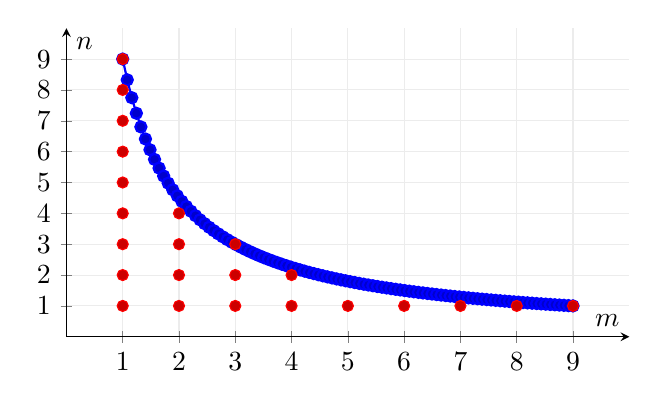
\begin{tikzpicture}
\begin{axis}[
    width=0.72\textwidth,
    height=5.5cm,
    axis lines=middle,
    xmin=0,
    xmax=10,
    ymin=0,
    ymax=10,
    xlabel={$m$},
    ylabel={$n$},
    xtick={1,2,...,9},
    ytick={1,2,...,9},
    grid=both,
    grid style={gray!15},
    domain=1:9,
    samples=100
]
\addplot+[thick] {9/x};
\addplot+[only marks,mark=*] coordinates {
(1,1)(1,2)(1,3)(1,4)(1,5)(1,6)(1,7)(1,8)(1,9)
(2,1)(2,2)(2,3)(2,4)
(3,1)(3,2)(3,3)
(4,1)(4,2)
(5,1)(6,1)(7,1)(8,1)(9,1)
};
\end{axis}
\end{tikzpicture}
\end{centereddiagram}

Estimating these lattice points leads to

\[ \sum_{n\leq x}\tau(n)=x\log x+(2\gamma-1)x+\Delta(x), \]

where \(\Delta(x)\) is an error term.

The symbol

\[ \gamma \]

is the Greek letter \emph{gamma}, pronounced ``GAM-uh.''

Here it denotes the Euler--Mascheroni constant,

\[ \gamma=\lim_{n\to\infty}\left(\sum_{k=1}^{n}\frac1k-\log n\right). \]

%%%%%%%%%%%%%%%%%%%%%%%%%%%%%%%%%%%%%%%%%%%%%%%%%%%%%%%%%%%%
\subsection{Dirichlet Series}
\label{subsec:dirichlet-series}
%%%%%%%%%%%%%%%%%%%%%%%%%%%%%%%%%%%%%%%%%%%%%%%%%%%%%%%%%%%%

Arithmetic functions can also be encoded by infinite series.

\begin{definitionbox}{Dirichlet Series}
A \emph{Dirichlet series} is an infinite series of the form

\[ \sum_{n=1}^{\infty}\frac{a(n)}{n^s}, \]

where \(a(n)\) is an arithmetic function and \(s\) is generally a complex
variable.
\end{definitionbox}

The variable

\[ s=\sigma+it \]

is commonly used in analytic number theory.

Here:

\begin{itemize}
    \item \(\sigma\) is the Greek letter sigma and denotes the real part;
    \item \(t\in\R\);
    \item \(i\) is the imaginary unit satisfying \(i^2=-1\).
\end{itemize}

Dirichlet series play a role similar to generating functions in
combinatorics.

%%%%%%%%%%%%%%%%%%%%%%%%%%%%%%%%%%%%%%%%%%%%%%%%%%%%%%%%%%%%
\subsection{The Riemann Zeta Function}
\label{subsec:riemann-zeta-function}
%%%%%%%%%%%%%%%%%%%%%%%%%%%%%%%%%%%%%%%%%%%%%%%%%%%%%%%%%%%%

The most famous Dirichlet series is the Riemann zeta function.

\begin{definitionbox}{Riemann Zeta Function}
For complex \(s\) satisfying

\[ \Re(s)>1, \]

the Riemann zeta function is defined by

\[ \boxed{\zeta(s)=\sum_{n=1}^{\infty}\frac{1}{n^s}.} \]
\end{definitionbox}

The symbol

\[ \zeta \]

is the Greek letter \emph{zeta}, commonly pronounced ``ZAY-tuh'' or
``ZEE-tuh.''

The notation

\[ \Re(s) \]

means the real part of the complex number \(s\).

For real \(s>1\),

\[ \zeta(s)=1+\frac1{2^s}+\frac1{3^s}+\frac1{4^s}+\cdots. \]

For example,

\[ \zeta(2)=\sum_{n=1}^{\infty}\frac1{n^2}=\frac{\pi^2}{6}. \]

%%%%%%%%%%%%%%%%%%%%%%%%%%%%%%%%%%%%%%%%%%%%%%%%%%%%%%%%%%%%
\subsection{Euler Product Formula}
\label{subsec:euler-product-formula}
%%%%%%%%%%%%%%%%%%%%%%%%%%%%%%%%%%%%%%%%%%%%%%%%%%%%%%%%%%%%

The connection between the zeta function and prime numbers is revealed by
Euler's product formula.

\begin{theorem}[Euler Product]
For

\[ \Re(s)>1, \]

the Riemann zeta function satisfies

\[ \boxed{\zeta(s)=\prod_{p\text{ prime}}\frac{1}{1-p^{-s}}.} \]
\end{theorem}

The symbol

\[ \prod \]

is the \emph{product symbol}, read ``the product.''

Thus

\[
\zeta(s)
=
\frac{1}{1-2^{-s}}
\frac{1}{1-3^{-s}}
\frac{1}{1-5^{-s}}
\frac{1}{1-7^{-s}}
\cdots.
\]

%%%%%%%%%%%%%%%%%%%%%%%%%%%%%%%%%%%%%%%%%%%%%%%%%%%%%%%%%%%%
\subsection{Why the Euler Product Works}
\label{subsec:euler-product-explanation}
%%%%%%%%%%%%%%%%%%%%%%%%%%%%%%%%%%%%%%%%%%%%%%%%%%%%%%%%%%%%

For each prime \(p\),

\[ \frac{1}{1-p^{-s}}=1+p^{-s}+p^{-2s}+p^{-3s}+\cdots. \]

Therefore

\[
\prod_p\frac{1}{1-p^{-s}}
=
\prod_p
\left(
1+p^{-s}+p^{-2s}+\cdots
\right).
\]

Expanding the product produces terms corresponding to products of prime
powers.

By the Fundamental Theorem of Arithmetic, every positive integer has exactly
one prime factorization. Consequently, every term

\[ \frac1{n^s} \]

appears exactly once.

Hence

\[ \prod_p\frac{1}{1-p^{-s}}=\sum_{n=1}^{\infty}\frac1{n^s}. \]

\begin{conceptbox}
The Euler product is an analytic expression of unique prime factorization:

\[
\boxed{
\text{unique factorization of integers}
\quad\Longleftrightarrow\quad
\text{Euler product for }\zeta(s)
}
\]

This is one of the fundamental bridges between algebraic arithmetic and
analysis.
\end{conceptbox}

%%%%%%%%%%%%%%%%%%%%%%%%%%%%%%%%%%%%%%%%%%%%%%%%%%%%%%%%%%%%
\subsection{Euler's Proof of Infinitely Many Primes Revisited}
\label{subsec:euler-infinite-primes-analytic}
%%%%%%%%%%%%%%%%%%%%%%%%%%%%%%%%%%%%%%%%%%%%%%%%%%%%%%%%%%%%

The Euler product provides an analytic perspective on the infinitude of
primes.

As \(s\to1^+\),

\[ \zeta(s)=\sum_{n=1}^{\infty}\frac1{n^s}\to\infty. \]

If only finitely many primes existed, the Euler product

\[ \prod_p\frac1{1-p^{-s}} \]

would contain only finitely many factors and would remain finite as
\(s\to1^+\).

This contradicts the divergence.

Therefore there must be infinitely many primes.

%%%%%%%%%%%%%%%%%%%%%%%%%%%%%%%%%%%%%%%%%%%%%%%%%%%%%%%%%%%%
\subsection{Logarithms of Euler Products}
\label{subsec:logarithms-euler-products}
%%%%%%%%%%%%%%%%%%%%%%%%%%%%%%%%%%%%%%%%%%%%%%%%%%%%%%%%%%%%

Taking logarithms transforms products over primes into sums over primes.

Starting with

\[ \zeta(s)=\prod_p(1-p^{-s})^{-1}, \]

we obtain

\[ \log\zeta(s)=-\sum_p\log(1-p^{-s}). \]

Using the power-series identity

\[ -\log(1-z)=\sum_{k=1}^{\infty}\frac{z^k}{k}, \]

we find

\[ \log\zeta(s)=\sum_p\sum_{k=1}^{\infty}\frac{1}{k p^{ks}}. \]

This illustrates a recurring analytic-number-theory strategy:

\[
\boxed{
\text{products over primes}
\longrightarrow
\text{logarithms}
\longrightarrow
\text{sums over prime powers}.
}
\]

%%%%%%%%%%%%%%%%%%%%%%%%%%%%%%%%%%%%%%%%%%%%%%%%%%%%%%%%%%%%
\subsection{The Logarithmic Derivative of \(\zeta\)}
\label{subsec:zeta-logarithmic-derivative}
%%%%%%%%%%%%%%%%%%%%%%%%%%%%%%%%%%%%%%%%%%%%%%%%%%%%%%%%%%%%

Differentiating the logarithm of the Euler product leads to the von Mangoldt
function.

For \(\Re(s)>1\),

\[ \boxed{-\frac{\zeta'(s)}{\zeta(s)}=\sum_{n=1}^{\infty}\frac{\Lambda(n)}{n^s}.} \]

The expression

\[ \frac{\zeta'(s)}{\zeta(s)} \]

is called the \emph{logarithmic derivative} of \(\zeta\).

This identity is central because it connects:

\[
\text{prime powers}
\longleftrightarrow
\Lambda(n)
\longleftrightarrow
-\frac{\zeta'(s)}{\zeta(s)}.
\]

%%%%%%%%%%%%%%%%%%%%%%%%%%%%%%%%%%%%%%%%%%%%%%%%%%%%%%%%%%%%
\subsection{Analytic Continuation of the Zeta Function}
\label{subsec:zeta-analytic-continuation}
%%%%%%%%%%%%%%%%%%%%%%%%%%%%%%%%%%%%%%%%%%%%%%%%%%%%%%%%%%%%

The series

\[ \sum_{n=1}^{\infty}\frac1{n^s} \]

converges absolutely only when

\[ \Re(s)>1. \]

However, complex analysis allows the zeta function to be extended beyond
this original domain.

\begin{theorem}[Analytic Continuation of \(\zeta\)]
The Riemann zeta function extends to a meromorphic function on the entire
complex plane, with a single simple pole at

\[ s=1. \]
\end{theorem}

The term \emph{meromorphic} means holomorphic except at isolated poles. This
concept is developed systematically in Complex Analysis.

\begin{warningbox}
Analytic continuation does not mean that the original infinite series

\[ \sum_{n=1}^{\infty}n^{-s} \]

converges everywhere.

Rather, another analytic function agrees with the series where the series
converges and extends the same function to a larger domain.
\end{warningbox}

%%%%%%%%%%%%%%%%%%%%%%%%%%%%%%%%%%%%%%%%%%%%%%%%%%%%%%%%%%%%
\subsection{The Functional Equation}
\label{subsec:zeta-functional-equation}
%%%%%%%%%%%%%%%%%%%%%%%%%%%%%%%%%%%%%%%%%%%%%%%%%%%%%%%%%%%%

The zeta function satisfies a remarkable symmetry.

One common form of its functional equation is

\[
\boxed{
\zeta(s)
=
2^s\pi^{s-1}
\sin\left(\frac{\pi s}{2}\right)
\Gamma(1-s)
\zeta(1-s).
}
\]

The symbol

\[ \Gamma \]

is the uppercase Greek letter \emph{gamma}.

Here

\[ \Gamma(z) \]

denotes the Gamma function, an extension of the factorial function.

For positive integers \(n\),

\[ \Gamma(n)=(n-1)!. \]

The functional equation connects values of the zeta function at \(s\) with
values at \(1-s\).

%%%%%%%%%%%%%%%%%%%%%%%%%%%%%%%%%%%%%%%%%%%%%%%%%%%%%%%%%%%%
\subsection{Zeros of the Zeta Function}
\label{subsec:zeta-zeros}
%%%%%%%%%%%%%%%%%%%%%%%%%%%%%%%%%%%%%%%%%%%%%%%%%%%%%%%%%%%%

A complex number \(s\) is a zero of the zeta function if

\[ \zeta(s)=0. \]

The functional equation produces zeros at the negative even integers

\[ -2,-4,-6,-8,\ldots. \]

These are called the \emph{trivial zeros}.

The remaining zeros are called \emph{nontrivial zeros}.

They lie in the region

\[ 0<\Re(s)<1, \]

called the \emph{critical strip}.

%%%%%%%%%%%%%%%%%%%%%%%%%%%%%%%%%%%%%%%%%%%%%%%%%%%%%%%%%%%%
\subsection{The Critical Strip}
\label{subsec:zeta-critical-strip}
%%%%%%%%%%%%%%%%%%%%%%%%%%%%%%%%%%%%%%%%%%%%%%%%%%%%%%%%%%%%

\begin{centereddiagram}
\begin{tikzpicture}[scale=0.9]
\draw[-{Latex[length=2.5mm]}] (-2.5,0)--(4.5,0)
    node[right] {\(\Re(s)\)};
\draw[-{Latex[length=2.5mm]}] (0,-3)--(0,3)
    node[above] {\(\Im(s)\)};

\fill[gray!12] (0,-2.7) rectangle (2,-0.05);
\fill[gray!12] (0,0.05) rectangle (2,2.7);

\draw[dashed] (0,-2.7)--(0,2.7);
\draw[dashed] (2,-2.7)--(2,2.7);
\draw[thick] (1,-2.7)--(1,2.7);

\node[below] at (0,0) {\(0\)};
\node[below] at (1,0) {\(\frac12\)};
\node[below] at (2,0) {\(1\)};

\node[rotate=90] at (1.7,1.6) {Critical strip};
\node[rotate=90] at (1.15,1.6) {Critical line};
\end{tikzpicture}
\end{centereddiagram}

The vertical line

\[ \Re(s)=\frac12 \]

is called the \emph{critical line}.

%%%%%%%%%%%%%%%%%%%%%%%%%%%%%%%%%%%%%%%%%%%%%%%%%%%%%%%%%%%%
\subsection{The Riemann Hypothesis}
\label{subsec:riemann-hypothesis}
%%%%%%%%%%%%%%%%%%%%%%%%%%%%%%%%%%%%%%%%%%%%%%%%%%%%%%%%%%%%

\begin{conjecture}[Riemann Hypothesis]
Every nontrivial zero of the Riemann zeta function has real part

\[ \boxed{\Re(s)=\frac12.} \]
\end{conjecture}

The Riemann Hypothesis is one of the most famous unsolved problems in
mathematics.

\begin{importantbox}
The Riemann Hypothesis is a conjecture, not a theorem.

It must never be used as an established fact unless a statement is explicitly
conditional on the hypothesis.
\end{importantbox}

Its importance comes largely from the relationship between zeros of
\(\zeta(s)\) and the error in approximations describing the distribution of
prime numbers.

%%%%%%%%%%%%%%%%%%%%%%%%%%%%%%%%%%%%%%%%%%%%%%%%%%%%%%%%%%%%
\subsection{Zeros and Prime Distribution}
\label{subsec:zeros-prime-distribution}
%%%%%%%%%%%%%%%%%%%%%%%%%%%%%%%%%%%%%%%%%%%%%%%%%%%%%%%%%%%%

The Prime Number Theorem gives the leading approximation

\[ \pi(x)\sim\frac{x}{\log x}. \]

More refined formulas reveal oscillations around the main approximation.

Very roughly,

\[
\boxed{
\text{zeros of }\zeta(s)
\quad\longleftrightarrow\quad
\text{fluctuations in the distribution of primes}.
}
\]

The real parts of the nontrivial zeros control the scale of important error
terms.

This is why a statement about zeros of a complex function can have profound
consequences for ordinary prime numbers.

%%%%%%%%%%%%%%%%%%%%%%%%%%%%%%%%%%%%%%%%%%%%%%%%%%%%%%%%%%%%
\subsection{The Harmonic Series over Primes}
\label{subsec:sum-reciprocals-primes}
%%%%%%%%%%%%%%%%%%%%%%%%%%%%%%%%%%%%%%%%%%%%%%%%%%%%%%%%%%%%

Although primes become less frequent, their reciprocals still form a
divergent series.

\begin{theorem}
The series

\[ \boxed{\sum_{p\text{ prime}}\frac1p} \]

diverges.
\end{theorem}

This result is stronger than merely proving that infinitely many primes
exist.

It shows that the primes are sufficiently numerous that their reciprocal
sum cannot converge.

%%%%%%%%%%%%%%%%%%%%%%%%%%%%%%%%%%%%%%%%%%%%%%%%%%%%%%%%%%%%
\subsection{Prime Number Races and Residue Classes}
\label{subsec:prime-residue-classes}
%%%%%%%%%%%%%%%%%%%%%%%%%%%%%%%%%%%%%%%%%%%%%%%%%%%%%%%%%%%%

The primes can also be studied according to their congruence classes.

For example, every prime \(p>2\) satisfies

\[ p\equiv1\pmod4 \]

or

\[ p\equiv3\pmod4. \]

This raises a natural question:

\begin{center}
Are there infinitely many primes in each allowed residue class?
\end{center}

The answer is yes in far greater generality.

%%%%%%%%%%%%%%%%%%%%%%%%%%%%%%%%%%%%%%%%%%%%%%%%%%%%%%%%%%%%
\subsection{Dirichlet's Theorem on Arithmetic Progressions}
\label{subsec:dirichlet-theorem-arithmetic-progressions}
%%%%%%%%%%%%%%%%%%%%%%%%%%%%%%%%%%%%%%%%%%%%%%%%%%%%%%%%%%%%

\begin{theorem}[Dirichlet's Theorem]
If

\[ \gcd(a,q)=1, \]

then there are infinitely many primes satisfying

\[ p\equiv a\pmod q. \]
\end{theorem}

Equivalently, the arithmetic progression

\[ a,\ a+q,\ a+2q,\ a+3q,\ldots \]

contains infinitely many primes whenever \(a\) and \(q\) are relatively
prime.

For example, there are infinitely many primes congruent to

\[ 1\pmod4 \]

and infinitely many primes congruent to

\[ 3\pmod4. \]

%%%%%%%%%%%%%%%%%%%%%%%%%%%%%%%%%%%%%%%%%%%%%%%%%%%%%%%%%%%%
\subsection{Why the Coprimality Condition Is Necessary}
\label{subsec:dirichlet-coprimality-condition}
%%%%%%%%%%%%%%%%%%%%%%%%%%%%%%%%%%%%%%%%%%%%%%%%%%%%%%%%%%%%

Suppose

\[ \gcd(a,q)>1. \]

Then \(a\) and \(q\) share a divisor \(d>1\).

Every term

\[ a+kq \]

is divisible by \(d\).

Therefore the progression cannot contain infinitely many primes.

For example,

\[ 6,10,14,18,22,\ldots \]

has the form

\[ 6+4k. \]

Every term is even, so only the first possible exceptional prime divisor can
occur; there cannot be infinitely many primes in the progression.

%%%%%%%%%%%%%%%%%%%%%%%%%%%%%%%%%%%%%%%%%%%%%%%%%%%%%%%%%%%%
\subsection{Dirichlet Characters}
\label{subsec:dirichlet-characters}
%%%%%%%%%%%%%%%%%%%%%%%%%%%%%%%%%%%%%%%%%%%%%%%%%%%%%%%%%%%%

To study primes in residue classes analytically, Dirichlet introduced special
periodic arithmetic functions.

\begin{definitionbox}{Dirichlet Character}
A \emph{Dirichlet character modulo \(q\)} is an arithmetic function
\(\chi\) that is periodic modulo \(q\), completely multiplicative, and
satisfies

\[ \chi(n)=0 \]

whenever

\[ \gcd(n,q)>1. \]
\end{definitionbox}

The symbol

\[ \chi \]

is the Greek letter \emph{chi}, commonly pronounced ``kye.''

The notation

\[ \chi(n) \]

is read ``chi of \(n\).''

Characters allow residue classes to be detected through algebraic and
analytic identities.

%%%%%%%%%%%%%%%%%%%%%%%%%%%%%%%%%%%%%%%%%%%%%%%%%%%%%%%%%%%%
\subsection{Example of a Dirichlet Character}
\label{subsec:dirichlet-character-example}
%%%%%%%%%%%%%%%%%%%%%%%%%%%%%%%%%%%%%%%%%%%%%%%%%%%%%%%%%%%%

Consider the function modulo \(4\),

\[
\chi(n)=
\begin{cases}
0, & n\text{ even},\\
1, & n\equiv1\pmod4,\\
-1, & n\equiv3\pmod4.
\end{cases}
\]

Then

\[ \chi(1)=1,\qquad\chi(3)=-1,\qquad\chi(5)=1,\qquad\chi(7)=-1. \]

The function distinguishes the two possible odd residue classes modulo \(4\).

%%%%%%%%%%%%%%%%%%%%%%%%%%%%%%%%%%%%%%%%%%%%%%%%%%%%%%%%%%%%
\subsection{Dirichlet \(L\)-Functions}
\label{subsec:dirichlet-l-functions}
%%%%%%%%%%%%%%%%%%%%%%%%%%%%%%%%%%%%%%%%%%%%%%%%%%%%%%%%%%%%

A Dirichlet character generates a Dirichlet series.

\begin{definitionbox}{Dirichlet \(L\)-Function}
For a Dirichlet character \(\chi\), define

\[ \boxed{L(s,\chi)=\sum_{n=1}^{\infty}\frac{\chi(n)}{n^s}} \]

for values of \(s\) where the series converges.
\end{definitionbox}

The notation

\[ L(s,\chi) \]

is read ``L of \(s\), chi.''

Like the zeta function, Dirichlet \(L\)-functions possess Euler products:

\[ \boxed{L(s,\chi)=\prod_p\frac{1}{1-\chi(p)p^{-s}}} \]

for \(\Re(s)>1\).

These functions allow analytic methods to distinguish primes in different
congruence classes.

%%%%%%%%%%%%%%%%%%%%%%%%%%%%%%%%%%%%%%%%%%%%%%%%%%%%%%%%%%%%
\subsection{The Zeta Function as an \(L\)-Function}
\label{subsec:zeta-as-l-function}
%%%%%%%%%%%%%%%%%%%%%%%%%%%%%%%%%%%%%%%%%%%%%%%%%%%%%%%%%%%%

The Riemann zeta function can be viewed as the simplest member of the broader
family of \(L\)-functions.

This leads to an important progression:

\[
\boxed{
\text{prime numbers}
\longrightarrow
\zeta(s)
\longrightarrow
L(s,\chi)
\longrightarrow
\text{general }L\text{-functions}.
}
\]

Modern number theory contains many families of \(L\)-functions associated
with arithmetic and geometric objects.

%%%%%%%%%%%%%%%%%%%%%%%%%%%%%%%%%%%%%%%%%%%%%%%%%%%%%%%%%%%%
\subsection{Partial Summation}
\label{subsec:partial-summation}
%%%%%%%%%%%%%%%%%%%%%%%%%%%%%%%%%%%%%%%%%%%%%%%%%%%%%%%%%%%%

A discrete analogue of integration by parts is extremely useful in analytic
number theory.

Let

\[ A(x)=\sum_{n\leq x}a_n. \]

Then, under appropriate hypotheses,

\[
\boxed{
\sum_{n\leq x}a_n f(n)
=
A(x)f(x)
-
\int_1^x A(t)f'(t)\,\dd t.
}
\]

This technique is called \emph{partial summation} or \emph{Abel summation}.

It allows information about the cumulative sum \(A(x)\) to be converted into
information about weighted sums.

%%%%%%%%%%%%%%%%%%%%%%%%%%%%%%%%%%%%%%%%%%%%%%%%%%%%%%%%%%%%
\subsection{Worked Example: Harmonic Numbers}
\label{subsec:worked-harmonic-asymptotic}
%%%%%%%%%%%%%%%%%%%%%%%%%%%%%%%%%%%%%%%%%%%%%%%%%%%%%%%%%%%%

The harmonic numbers are

\[ H_n=\sum_{k=1}^{n}\frac1k. \]

Their growth satisfies

\[ H_n=\log n+\gamma+O\left(\frac1n\right). \]

Thus

\[ H_n\sim\log n. \]

This is a simple example of an exact finite arithmetic sum being approximated
by an analytic function.

%%%%%%%%%%%%%%%%%%%%%%%%%%%%%%%%%%%%%%%%%%%%%%%%%%%%%%%%%%%%
\subsection{Average Order}
\label{subsec:average-order}
%%%%%%%%%%%%%%%%%%%%%%%%%%%%%%%%%%%%%%%%%%%%%%%%%%%%%%%%%%%%

Arithmetic functions can fluctuate greatly from integer to integer.

Rather than studying \(f(n)\) individually, one may study

\[ \frac1x\sum_{n\leq x}f(n). \]

This represents an average value of \(f\) up to \(x\).

For example, the divisor-counting function \(\tau(n)\) has average order

\[ \log n. \]

More precisely,

\[ \sum_{n\leq x}\tau(n)=x\log x+(2\gamma-1)x+O(\sqrt{x}). \]

Thus, on average, an integer near \(x\) has roughly \(\log x\) positive
divisors.

%%%%%%%%%%%%%%%%%%%%%%%%%%%%%%%%%%%%%%%%%%%%%%%%%%%%%%%%%%%%
\subsection{Normal Order}
\label{subsec:normal-order}
%%%%%%%%%%%%%%%%%%%%%%%%%%%%%%%%%%%%%%%%%%%%%%%%%%%%%%%%%%%%

Average behavior can sometimes be distorted by unusually large or small
values.

A \emph{normal order} describes the typical size of an arithmetic function
for almost all integers.

This distinction between

\[
\text{average behavior}
\qquad\text{and}\qquad
\text{typical behavior}
\]

becomes important in probabilistic number theory.

%%%%%%%%%%%%%%%%%%%%%%%%%%%%%%%%%%%%%%%%%%%%%%%%%%%%%%%%%%%%
\subsection{Prime Gaps}
\label{subsec:prime-gaps}
%%%%%%%%%%%%%%%%%%%%%%%%%%%%%%%%%%%%%%%%%%%%%%%%%%%%%%%%%%%%

Let

\[ p_1<p_2<p_3<\cdots \]

denote the primes in increasing order.

The quantity

\[ g_n=p_{n+1}-p_n \]

is called the \(n\)-th \emph{prime gap}.

For example,

\[ 2,3,5,7,11,13 \]

give gaps

\[ 1,2,2,4,2. \]

Prime gaps are highly irregular.

The Prime Number Theorem suggests that a typical gap near \(x\) should have
scale roughly

\[ \log x. \]

However, individual gaps can behave very differently from this average
scale.

%%%%%%%%%%%%%%%%%%%%%%%%%%%%%%%%%%%%%%%%%%%%%%%%%%%%%%%%%%%%
\subsection{Twin Primes}
\label{subsec:twin-primes}
%%%%%%%%%%%%%%%%%%%%%%%%%%%%%%%%%%%%%%%%%%%%%%%%%%%%%%%%%%%%

\begin{definitionbox}{Twin Primes}
A pair of primes of the form

\[ p,\qquad p+2 \]

is called a pair of \emph{twin primes}.
\end{definitionbox}

Examples include

\[ (3,5),\qquad(5,7),\qquad(11,13),\qquad(17,19). \]

The Twin Prime Conjecture asserts that infinitely many such pairs exist.

\begin{conjecture}[Twin Prime Conjecture]
There are infinitely many primes \(p\) such that \(p+2\) is also prime.
\end{conjecture}

This remains unresolved.

%%%%%%%%%%%%%%%%%%%%%%%%%%%%%%%%%%%%%%%%%%%%%%%%%%%%%%%%%%%%
\subsection{Goldbach's Conjecture}
\label{subsec:goldbach-conjecture}
%%%%%%%%%%%%%%%%%%%%%%%%%%%%%%%%%%%%%%%%%%%%%%%%%%%%%%%%%%%%

Another famous unresolved problem concerns additive prime structure.

\begin{conjecture}[Goldbach's Conjecture]
Every even integer greater than \(2\) can be written as the sum of two prime
numbers.
\end{conjecture}

Examples include

\[ 10=3+7,\qquad20=7+13,\qquad100=47+53. \]

Goldbach's Conjecture illustrates the distinction between multiplicative and
additive number theory.

%%%%%%%%%%%%%%%%%%%%%%%%%%%%%%%%%%%%%%%%%%%%%%%%%%%%%%%%%%%%
\subsection{Multiplicative and Additive Number Theory}
\label{subsec:multiplicative-additive-number-theory}
%%%%%%%%%%%%%%%%%%%%%%%%%%%%%%%%%%%%%%%%%%%%%%%%%%%%%%%%%%%%

Multiplicative number theory studies structures involving products and
divisibility, such as

\[
\text{primes},\quad
\varphi(n),\quad
\mu(n),\quad
\tau(n),\quad
\zeta(s).
\]

Additive number theory studies representations involving sums, such as

\[ n=p_1+p_2 \]

or more generally

\[ n=a_1+\cdots+a_k. \]

Analytic methods are powerful in both settings.

%%%%%%%%%%%%%%%%%%%%%%%%%%%%%%%%%%%%%%%%%%%%%%%%%%%%%%%%%%%%
\subsection{The Circle Method}
\label{subsec:circle-method-introduction}
%%%%%%%%%%%%%%%%%%%%%%%%%%%%%%%%%%%%%%%%%%%%%%%%%%%%%%%%%%%%

A major technique in additive number theory is the \emph{circle method}.

Very roughly, the method transforms an arithmetic counting problem into an
integral involving generating functions on the complex unit circle.

The general philosophy is

\[
\boxed{
\text{count integer representations}
\longrightarrow
\text{construct generating function}
\longrightarrow
\text{integrate analytically}.
}
\]

The full method requires Fourier and complex analysis and is therefore only
introduced conceptually here.

%%%%%%%%%%%%%%%%%%%%%%%%%%%%%%%%%%%%%%%%%%%%%%%%%%%%%%%%%%%%
\subsection{Sieve Methods}
\label{subsec:sieve-methods-introduction}
%%%%%%%%%%%%%%%%%%%%%%%%%%%%%%%%%%%%%%%%%%%%%%%%%%%%%%%%%%%%

A sieve removes integers divisible by selected primes in order to isolate or
estimate integers having desired arithmetic properties.

The classical model is the Sieve of Eratosthenes.

\begin{centereddiagram}
\begin{tikzpicture}[
    cell/.style={draw,minimum width=0.72cm,minimum height=0.55cm}
]
\foreach \n in {1,...,30}{
    \pgfmathtruncatemacro{\row}{int((\n-1)/10)}
    \pgfmathtruncatemacro{\col}{mod(\n-1,10)}
    \node[cell] (n\n) at (\col*0.72,-\row*0.55) {\scriptsize \n};
}

\foreach \p in {2,3,5,7,11,13,17,19,23,29}{
    \node[draw=MathBlue,line width=0.8pt,rounded corners,
    fit=(n\p),inner sep=0pt] {};
}
\end{tikzpicture}
\end{centereddiagram}

Modern sieve methods do not merely list primes. They produce quantitative
estimates for sets defined by divisibility restrictions.

%%%%%%%%%%%%%%%%%%%%%%%%%%%%%%%%%%%%%%%%%%%%%%%%%%%%%%%%%%%%
\subsection{Analytic Number Theory and Complex Analysis}
\label{subsec:analytic-number-theory-complex-analysis}
%%%%%%%%%%%%%%%%%%%%%%%%%%%%%%%%%%%%%%%%%%%%%%%%%%%%%%%%%%%%

Complex analysis becomes one of the central tools of analytic number theory.

Functions such as

\[ \zeta(s) \]

and

\[ L(s,\chi) \]

are studied through:

\begin{itemize}
    \item analytic continuation;
    \item poles and zeros;
    \item contour integration;
    \item residue calculus;
    \item functional equations;
    \item growth estimates.
\end{itemize}

This produces a remarkable bridge:

\[
\boxed{
\text{discrete integers}
\longleftrightarrow
\text{complex analytic functions}.
}
\]

%%%%%%%%%%%%%%%%%%%%%%%%%%%%%%%%%%%%%%%%%%%%%%%%%%%%%%%%%%%%
\subsection{Common Errors}
\label{subsec:analytic-number-theory-common-errors}
%%%%%%%%%%%%%%%%%%%%%%%%%%%%%%%%%%%%%%%%%%%%%%%%%%%%%%%%%%%%

\subsubsection{Confusing \(\pi(x)\) with the Constant \(\pi\)}

In analytic number theory,

\[ \pi(x) \]

usually denotes the number of primes not exceeding \(x\).

The constant

\[ \pi=3.14159\ldots \]

is a different object.

%%%%%%%%%%%%%%%%%%%%%%%%%%%%%%%%%%%%%%%%%%%%%%%%%%%%%%%%%%%%
\subsubsection{Interpreting the Prime Number Theorem as Exact}

The statement

\[ \pi(x)\sim\frac{x}{\log x} \]

does not mean

\[ \pi(x)=\frac{x}{\log x}. \]

The theorem describes asymptotic behavior.

%%%%%%%%%%%%%%%%%%%%%%%%%%%%%%%%%%%%%%%%%%%%%%%%%%%%%%%%%%%%
\subsubsection{Assuming \(x/\log x\) Is Always a Very Accurate Estimate}

The relative error tends to zero only as

\[ x\to\infty. \]

For modest \(x\), the approximation can still differ noticeably from the
actual value.

%%%%%%%%%%%%%%%%%%%%%%%%%%%%%%%%%%%%%%%%%%%%%%%%%%%%%%%%%%%%
\subsubsection{Confusing Multiplicative and Completely Multiplicative}

A multiplicative function requires

\[ f(mn)=f(m)f(n) \]

only when

\[ \gcd(m,n)=1. \]

A completely multiplicative function satisfies the identity without the
coprimality condition.

%%%%%%%%%%%%%%%%%%%%%%%%%%%%%%%%%%%%%%%%%%%%%%%%%%%%%%%%%%%%
\subsubsection{Confusing Ordinary Multiplication with Dirichlet Convolution}

The notation

\[ f*g \]

does not generally mean pointwise multiplication.

It means

\[ (f*g)(n)=\sum_{d\mid n}f(d)g(n/d). \]

%%%%%%%%%%%%%%%%%%%%%%%%%%%%%%%%%%%%%%%%%%%%%%%%%%%%%%%%%%%%
\subsubsection{Using the Euler Product Outside Its Initial Region}

The identity

\[ \zeta(s)=\prod_p(1-p^{-s})^{-1} \]

is directly convergent in the region

\[ \Re(s)>1. \]

Analytic continuation does not automatically justify every manipulation of
the product outside this region.

%%%%%%%%%%%%%%%%%%%%%%%%%%%%%%%%%%%%%%%%%%%%%%%%%%%%%%%%%%%%
\subsubsection{Confusing Analytic Continuation with Series Convergence}

The analytically continued zeta function exists at many points where

\[ \sum_{n=1}^{\infty}n^{-s} \]

does not converge.

These are not the same statement.

%%%%%%%%%%%%%%%%%%%%%%%%%%%%%%%%%%%%%%%%%%%%%%%%%%%%%%%%%%%%
\subsubsection{Treating the Riemann Hypothesis as Proven}

The Riemann Hypothesis remains unproved.

Any result depending on it must be explicitly described as conditional.

%%%%%%%%%%%%%%%%%%%%%%%%%%%%%%%%%%%%%%%%%%%%%%%%%%%%%%%%%%%%
\subsubsection{Assuming Prime Density Means Regular Spacing}

The heuristic density

\[ \frac1{\log x} \]

does not imply that primes occur every \(\log x\) integers.

Prime gaps fluctuate substantially.

%%%%%%%%%%%%%%%%%%%%%%%%%%%%%%%%%%%%%%%%%%%%%%%%%%%%%%%%%%%%
\subsubsection{Assuming Dirichlet's Theorem Covers Every Arithmetic Progression}

The condition

\[ \gcd(a,q)=1 \]

is essential.

Without it, the progression can have a fixed nontrivial divisor.

%%%%%%%%%%%%%%%%%%%%%%%%%%%%%%%%%%%%%%%%%%%%%%%%%%%%%%%%%%%%
\subsection{Applications and Connections}
\label{subsec:analytic-number-theory-applications}
%%%%%%%%%%%%%%%%%%%%%%%%%%%%%%%%%%%%%%%%%%%%%%%%%%%%%%%%%%%%

\begin{applicationbox}
\textbf{Prime Distribution.}
The Prime Number Theorem describes the large-scale density of primes and is
one of the foundational results of analytic number theory.

\medskip

\textbf{Complex Analysis.}
The Riemann zeta function and Dirichlet \(L\)-functions connect arithmetic
questions to zeros, poles, analytic continuation, and contour integration.

\medskip

\textbf{Fourier Analysis.}
Fourier methods appear naturally in additive number theory, exponential
sums, and the circle method.

\medskip

\textbf{Probability.}
Arithmetic functions often exhibit statistical behavior, motivating
probabilistic models for prime factors and other number-theoretic quantities.

\medskip

\textbf{Cryptography.}
Estimates concerning primes influence the generation and availability of
large primes used in computational applications.

\medskip

\textbf{Algebraic Number Theory.}
Generalizations of the zeta function arise from number fields and other
algebraic structures.

\medskip

\textbf{Arithmetic Geometry.}
More advanced \(L\)-functions encode information about algebraic varieties,
elliptic curves, and other arithmetic-geometric objects.

\medskip

\textbf{Computational Number Theory.}
Analytic estimates help predict the complexity and expected behavior of
algorithms involving primes and arithmetic functions.
\end{applicationbox}

%%%%%%%%%%%%%%%%%%%%%%%%%%%%%%%%%%%%%%%%%%%%%%%%%%%%%%%%%%%%
\subsection{Exercises}
\label{subsec:analytic-number-theory-exercises}
%%%%%%%%%%%%%%%%%%%%%%%%%%%%%%%%%%%%%%%%%%%%%%%%%%%%%%%%%%%%

\begin{exercise}[1]
Compute

\[ \pi(10),\qquad\pi(20),\qquad\pi(50),\qquad\pi(100). \]
\end{exercise}

\begin{exercise}[1]
Use

\[ \frac{x}{\log x} \]

to estimate \(\pi(1000)\).
\end{exercise}

\begin{exercise}[2]
Compare the approximation

\[ \frac{x}{\log x} \]

with the actual value

\[ \pi(1000)=168. \]

Compute the absolute error.
\end{exercise}

\begin{exercise}[2]
Compute the relative error of the approximation in the previous exercise.
\end{exercise}

\begin{exercise}[2]
Explain in words what

\[ \pi(x)\sim\frac{x}{\log x} \]

means.
\end{exercise}

\begin{exercise}[2]
Show that

\[ x+1\sim x. \]
\end{exercise}

\begin{exercise}[2]
Show that

\[ x^2+x=O(x^2). \]
\end{exercise}

\begin{exercise}[2]
Show that

\[ \log x=o(x). \]
\end{exercise}

\begin{exercise}[1]
Compute

\[ \mu(1),\ \mu(2),\ \mu(4),\ \mu(6),\ \mu(12),\ \mu(30),\ \mu(42). \]
\end{exercise}

\begin{exercise}[2]
Verify that

\[ \sum_{d\mid10}\mu(d)=0. \]
\end{exercise}

\begin{exercise}[2]
Verify that

\[ \sum_{d\mid30}\mu(d)=0. \]
\end{exercise}

\begin{exercise}[2]
Determine whether each function is multiplicative:

\[
f(n)=1,\qquad
f(n)=n,\qquad
f(n)=n^2.
\]
\end{exercise}

\begin{exercise}[2]
Compute

\[ (\mathbf{1}*\mathbf{1})(12) \]

directly from the definition of Dirichlet convolution.
\end{exercise}

\begin{exercise}[2]
Verify that

\[ (\mu*\mathbf{1})(6)=0. \]
\end{exercise}

\begin{exercise}[3]
Use Möbius inversion on

\[ n=\sum_{d\mid n}\varphi(d) \]

to derive

\[ \varphi(n)=\sum_{d\mid n}\mu(d)\frac nd. \]
\end{exercise}

\begin{exercise}[1]
Compute

\[ \Lambda(2),\quad\Lambda(4),\quad\Lambda(6),\quad\Lambda(8),\quad\Lambda(9). \]
\end{exercise}

\begin{exercise}[2]
Compute

\[ \psi(10)=\sum_{n\leq10}\Lambda(n). \]
\end{exercise}

\begin{exercise}[2]
Write the first five terms of

\[ \zeta(2)=\sum_{n=1}^{\infty}\frac1{n^2}. \]
\end{exercise}

\begin{exercise}[2]
Write the first four prime factors in the Euler product for

\[ \zeta(2). \]
\end{exercise}

\begin{exercise}[3]
Explain how the Fundamental Theorem of Arithmetic leads to the Euler product

\[ \zeta(s)=\prod_p(1-p^{-s})^{-1}. \]
\end{exercise}

\begin{exercise}[2]
Explain why the Euler product provides another proof that infinitely many
primes exist.
\end{exercise}

\begin{exercise}[2]
What is the difference between the original Dirichlet series defining
\(\zeta(s)\) and the analytic continuation of \(\zeta(s)\)?
\end{exercise}

\begin{exercise}[1]
List the first five trivial zeros of the Riemann zeta function.
\end{exercise}

\begin{exercise}[2]
Describe the critical strip and critical line.
\end{exercise}

\begin{exercise}[2]
State the Riemann Hypothesis without claiming that it has been proved.
\end{exercise}

\begin{exercise}[2]
Explain conceptually why zeros of the zeta function can affect estimates for
prime-counting functions.
\end{exercise}

\begin{exercise}[1]
List the first five primes congruent to

\[ 1\pmod4. \]
\end{exercise}

\begin{exercise}[1]
List the first five primes congruent to

\[ 3\pmod4. \]
\end{exercise}

\begin{exercise}[2]
Determine whether Dirichlet's theorem guarantees infinitely many primes in

\[ 5+6k. \]
\end{exercise}

\begin{exercise}[2]
Determine whether Dirichlet's theorem guarantees infinitely many primes in

\[ 6+9k. \]

Explain.
\end{exercise}

\begin{exercise}[2]
For the character modulo \(4\) defined in this section, compute

\[ \chi(9),\qquad\chi(11),\qquad\chi(14),\qquad\chi(17). \]
\end{exercise}

\begin{exercise}[2]
Write the first six terms of

\[ L(s,\chi)=\sum_{n=1}^{\infty}\frac{\chi(n)}{n^s} \]

for the nonprincipal character modulo \(4\).
\end{exercise}

\begin{exercise}[2]
Calculate the first six prime gaps.
\end{exercise}

\begin{exercise}[1]
Give five examples of twin-prime pairs.
\end{exercise}

\begin{exercise}[2]
Explain why the Twin Prime Conjecture is stronger than the statement that
there are infinitely many primes.
\end{exercise}

\begin{exercise}[2]
Write five even integers greater than \(2\) as sums of two primes.
\end{exercise}

\begin{exercise}[2]
Explain the difference between multiplicative and additive number theory.
\end{exercise}

\begin{exercise}[3]
Show that

\[ \sum_{n\leq x}\tau(n) \]

counts the positive integer lattice points satisfying

\[ ab\leq x. \]
\end{exercise}

\begin{exercise}[3]
Explain why Dirichlet series are analogous to generating functions even
though their terms involve \(n^{-s}\) rather than powers \(x^n\).
\end{exercise}

\begin{exercise}[3]
Explain the conceptual chain

\[
\text{integers}
\longrightarrow
\text{arithmetic functions}
\longrightarrow
\text{Dirichlet series}
\longrightarrow
\text{complex functions}
\longrightarrow
\text{information about integers}.
\]
\end{exercise}

%%%%%%%%%%%%%%%%%%%%%%%%%%%%%%%%%%%%%%%%%%%%%%%%%%%%%%%%%%%%
\subsection{Conceptual Summary}
\label{subsec:analytic-number-theory-summary}
%%%%%%%%%%%%%%%%%%%%%%%%%%%%%%%%%%%%%%%%%%%%%%%%%%%%%%%%%%%%

Analytic number theory uses analytic methods to study arithmetic structure.

The prime-counting function

\[ \pi(x)=\#\{p\leq x:p\text{ prime}\} \]

records the number of primes up to \(x\).

The Prime Number Theorem states

\[ \boxed{\pi(x)\sim\frac{x}{\log x}}, \]

showing that the approximate density of primes near \(x\) is

\[ \frac1{\log x}. \]

Arithmetic functions encode structural information about integers.
Important examples include

\[ \varphi(n),\qquad\tau(n),\qquad\sigma(n),\qquad\mu(n),\qquad\Lambda(n). \]

Dirichlet convolution

\[ (f*g)(n)=\sum_{d\mid n}f(d)g(n/d) \]

provides an algebra adapted to divisor sums, while Möbius inversion allows
such sums to be reversed.

Dirichlet series encode arithmetic functions analytically.

The central example is

\[ \zeta(s)=\sum_{n=1}^{\infty}\frac1{n^s}. \]

The Euler product

\[ \boxed{\zeta(s)=\prod_p(1-p^{-s})^{-1}} \]

connects the zeta function directly to prime factorization.

Analytic continuation extends the zeta function beyond the original region
of convergence, while its zeros contain information about fluctuations in
prime distribution.

The Riemann Hypothesis predicts that every nontrivial zero satisfies

\[ \Re(s)=\frac12, \]

but this remains an open problem.

Dirichlet characters and \(L\)-functions extend analytic methods to primes in
arithmetic progressions.

Together, these ideas demonstrate one of the deepest recurring principles in
mathematics:

\[
\boxed{
\text{discrete arithmetic structure can be studied through continuous and
complex analytic objects}.
}
\]

%%%%%%%%%%%%%%%%%%%%%%%%%%%%%%%%%%%%%%%%%%%%%%%%%%%%%%%%%%%%
\subsection{Section Connections}
\label{subsec:analytic-number-theory-connections}
%%%%%%%%%%%%%%%%%%%%%%%%%%%%%%%%%%%%%%%%%%%%%%%%%%%%%%%%%%%%

\chapterconnection{
Analytic Number Theory builds on the divisibility, prime numbers,
congruences, and arithmetic functions introduced in Elementary Number
Theory. The Prime Number Theorem begins the systematic study of prime
distribution. Dirichlet series transform arithmetic functions into analytic
objects, while the Euler product translates unique prime factorization into
an infinite product. The Riemann zeta function provides a major bridge to
Real Analysis, Complex Analysis, Fourier Analysis, and Asymptotic Analysis.
Dirichlet characters and \(L\)-functions connect congruence classes with
complex analysis and prepare the reader for deeper results concerning primes
in arithmetic progressions. Generalizations of zeta and \(L\)-functions
appear throughout Algebraic Number Theory and Arithmetic Geometry.
Probabilistic questions about arithmetic functions lead toward Probabilistic
Number Theory, while numerical investigation of primes and zeta functions
connects with Computational Number Theory.
}

%%%%%%%%%%%%%%%%%%%%%%%%%%%%%%%%%%%%%%%%%%%%%%%%%%%%%%%%%%%%
% SECTION SOURCE TRACKING
%%%%%%%%%%%%%%%%%%%%%%%%%%%%%%%%%%%%%%%%%%%%%%%%%%%%%%%%%%%%

%------------------------------------------------------------
% 2.2 Analytic Number Theory
%------------------------------------------------------------
%
% Source basis:
%   - Standard undergraduate and introductory graduate analytic
%     number theory.
%
% Used for:
%   - prime-counting function;
%   - asymptotic equivalence;
%   - Prime Number Theorem;
%   - logarithmic integral;
%   - Chebyshev functions;
%   - von Mangoldt function;
%   - Möbius function;
%   - multiplicative functions;
%   - Dirichlet convolution;
%   - Möbius inversion;
%   - summatory functions;
%   - asymptotic notation;
%   - divisor problem and hyperbola method;
%   - Dirichlet series;
%   - Riemann zeta function;
%   - Euler product;
%   - logarithmic derivative of zeta;
%   - analytic continuation and functional equation;
%   - trivial and nontrivial zeros;
%   - critical strip and Riemann Hypothesis;
%   - primes in arithmetic progressions;
%   - Dirichlet characters and L-functions;
%   - partial summation;
%   - average order;
%   - prime gaps and twin primes;
%   - additive number theory;
%   - introductory sieve and circle-method viewpoints.
%
% Notes:
%   - Elementary divisibility and congruence theory are taught
%     canonically in Section 2.1.
%   - Rigorous real-analysis foundations are taught in Chapter 5.
%   - Complex differentiation, analytic continuation, contour
%     integration, and residue theory are taught canonically in
%     Complex Analysis.
%   - Fourier-analytic machinery is taught canonically in
%     Fourier Analysis.
%   - Advanced computational algorithms are deferred to
%     Computational Number Theory.
%   - Probabilistic models of arithmetic functions are deferred
%     to Probabilistic Number Theory.
%   - Number-field zeta functions and deeper L-functions are
%     developed in Algebraic Number Theory and Arithmetic Geometry.
%
%%%%%%%%%%%%%%%%%%%%%%%%%%%%%%%%%%%%%%%%%%%%%%%%%%%%%%%%%%%%